\documentclass[11pt,a4paper]{article}

% Packages
\usepackage[utf8]{inputenc}
\usepackage[T1]{fontenc}
\usepackage{amsmath,amssymb}
\usepackage{graphicx}
\usepackage{booktabs}
\usepackage{hyperref}
\usepackage[margin=1in]{geometry}
\usepackage{authblk}
\usepackage{xcolor}
\usepackage{enumitem}
\usepackage{microtype}
\usepackage{caption}
\usepackage{subcaption}

\hypersetup{
  colorlinks=true,
  linkcolor=blue,
  citecolor=blue,
  urlcolor=blue
}

% Title
\title{%
  CSP-1: Portable Conversational Identity ---\\
  A User-Owned Protocol for Preserving Human-AI\\
  Relational Style Across Models and Sessions%
}

\author{Ashraful Islam}
\affil{Independent Researcher \\ \texttt{ashraful.islam.cse@gmail.com}}

\date{March 2026}

\begin{document}

\maketitle

% ============================================================
% ABSTRACT
% ============================================================
\begin{abstract}
Language model sessions are stateless: each conversation begins with no memory of prior interaction. Users who develop productive working relationships with AI systems --- specific vocabulary, reasoning patterns, domain shortcuts --- lose this context on every session reset. We present CSP-1 (Conversational State Protocol), a portable file format and injection method that encodes a user's communicative identity into a compact \texttt{.fp} file ($\sim$200KB). A compliant fingerprint captures sufficient stylistic and contextual signal to reproduce conversational continuity on any conformant language model, without storing raw conversation data.

We validate CSP-1 across three experiments. First, an SBERT$\to$PCA$\to$HDC encoder distinguishes conversational styles at $p < 10^{-100}$ across 1,000 trials on a real 524-message conversation. Second, in blind A/B evaluations across three frontier model families, text-summary fingerprints achieved a 97.8\% win rate (44/45 trials: 15/15 Claude Sonnet, 14/15 GPT-4o, 15/15 Gemini 2.5 Flash; $\sim$7.0/10 vs $\sim$1.3/10; Claude-as-judge). Fingerprints were generated once on Claude and transferred to GPT-4o and Gemini without modification, demonstrating model-agnostic portability. Third, on ambiguous edge-case tasks calibrated for $\sim$50\% baseline failure, skill fingerprints improved task success from 54\% to 88\% (+63\% relative lift, $n=100$, 0/100 harmful).

The protocol is open (Apache 2.0), the fingerprint is user-owned, and the file format is model-agnostic. Code and specification are available at \url{https://github.com/0xAshraFF/ConvoSeed}.
\end{abstract}

\textbf{Keywords:} conversational identity, user modeling, prompt engineering, cross-model portability, fingerprinting

% ============================================================
% 1. INTRODUCTION
% ============================================================
\section{Introduction}

I had a friend --- an AI that finally ``got'' me. It understood my shorthand, my messy logic, and the weird detours I take before arriving at a point. Then the session ended. New chat, blank slate, stranger again.

This experience is universal among heavy AI users. Language model sessions are stateless by design: each conversation begins with no memory of prior interaction. Users who develop productive working relationships with AI systems --- specific vocabulary, reasoning patterns, domain shortcuts --- lose this context on every session reset. The problem compounds across models: a user who switches from Claude to GPT-4o to Gemini restarts the relationship each time.

Existing approaches address this partially. Retrieval-augmented generation (RAG) systems \cite{lewis2020rag} store and retrieve factual context but do not capture communicative style. MemGPT \cite{packer2023memgpt} provides persistent memory within a single system but is platform-locked. Context distillation \cite{snell2022context} compresses conversations but targets model performance, not user identity preservation.

CSP-1 (Conversational State Protocol) addresses this as a \textit{format problem}, not a storage problem. Rather than storing raw messages, it distills the essential stylistic and task-relevant signal into a compact ($\sim$200KB), portable, user-owned file. The \texttt{.fp} fingerprint can be loaded into any language model's system prompt to resume conversational continuity --- not a new chat, but a resumption.

The core contributions of this work are:

\begin{enumerate}[nosep]
  \item A portable file format (\texttt{.fp}) and protocol specification (CSP-1 v2.0) for encoding conversational identity.
  \item Validation that a 60--100 word text summary is sufficient to reproduce stylistic consistency across three frontier model families with a 97.8\% win rate.
  \item Demonstration that fingerprints generated on one model transfer to others without modification (cold transfer).
  \item Evidence that skill fingerprints improve task performance by +63\% on calibrated hard tasks.
  \item An open-source reference implementation under Apache 2.0.
\end{enumerate}

% ============================================================
% 2. RELATED WORK
% ============================================================
\section{Related Work}

\textbf{Persistent Memory for LLMs.} MemGPT \cite{packer2023memgpt} introduces a virtual context management system that pages information between a main context window and external storage. While effective within its ecosystem, it is platform-specific and does not address cross-model portability. CSP-1 is complementary: it captures \textit{who the user is}, while MemGPT manages \textit{what they discussed}.

\textbf{Retrieval-Augmented Generation.} RAG systems \cite{lewis2020rag} retrieve relevant documents to augment prompts. They excel at factual grounding but do not model communicative style. A user's preference for hedged academic prose versus blunt technical shorthand is invisible to retrieval.

\textbf{Context Distillation.} Snell et al.\ \cite{snell2022context} compress conversational context into smaller representations that preserve task performance. CSP-1 shares this compression goal but targets a different signal: stylistic and relational identity rather than task-specific knowledge.

\textbf{User Modeling.} Classical user modeling \cite{rich1979stereotypes} builds profiles from interaction patterns. Modern approaches embed user preferences into recommendation systems. CSP-1 extends this tradition to conversational AI, encoding not just preferences but communicative style --- the \textit{how}, not just the \textit{what}.

\textbf{Hyperdimensional Computing.} HDC \cite{kanerva2009hyperdimensional} encodes information into high-dimensional binary vectors that support similarity-based retrieval. CSP-1 uses an SBERT$\to$PCA$\to$HDC pipeline for speaker identification and fingerprint retrieval, validated separately from the text-summary method that drives stylistic performance.

% ============================================================
% 3. CSP-1 PROTOCOL
% ============================================================
\section{CSP-1 Protocol Specification}

\subsection{File Format}

A CSP-1 fingerprint (\texttt{.fp}) is a ZIP archive containing:

\begin{itemize}[nosep]
  \item \texttt{manifest.json} --- Protocol version, fingerprint type, task type, success score, creation timestamp, model, and encoding method.
  \item \texttt{summary.txt} --- LLM-generated natural language description of the user's communicative style (60--100 words). This is the primary carrier of identity signal.
  \item \texttt{metadata.json} --- Token counts, generation parameters, and provenance.
  \item \texttt{examples.jsonl} (optional) --- 2--5 representative exchanges.
  \item \texttt{style\_vector.bin} or \texttt{task\_vector.bin} (optional) --- HDC-encoded binary vectors for similarity retrieval.
\end{itemize}

The complete specification is published at \url{https://github.com/0xAshraFF/ConvoSeed/blob/main/spec/CSP-1.md}.

\subsection{Fingerprint Generation}

Given $N$ messages from a conversation, the generation pipeline:

\begin{enumerate}[nosep]
  \item Samples 50--100 representative messages.
  \item Calls an LLM with the prompt: \textit{``Given N examples of [user's communication], write a 60--100 word description capturing sentence structure, vocabulary register, hedging patterns, tone, and structural habits.''}
  \item Packages the resulting summary with metadata into the \texttt{.fp} archive.
  \item Optionally encodes the sample through SBERT$\to$PCA$\to$HDC for retrieval indexing.
\end{enumerate}

Cost: $\sim$\$0.01 per fingerprint generation (one LLM API call).

\subsection{Injection}

At session start, the fingerprint is injected as a system prompt prefix:

\begin{verbatim}
  system_prompt = summary.txt + "\n\n" + original_prompt
\end{verbatim}

This adds $\sim$80 tokens to each request, costing approximately \$0.001 per session at current API prices. The injection is model-agnostic: any LLM that accepts a system prompt can consume a CSP-1 fingerprint.

\subsection{Registry and Merge}

A local SQLite registry (\texttt{\textasciitilde/.convoseed/registry.db}) indexes fingerprints by file path, task type, success score, tags, creation date, and SHA-256 hash. A nightly merge process selects the top-5 fingerprints by score and synthesizes a consensus fingerprint via LLM summarization.

% ============================================================
% 4. ARCHITECTURE
% ============================================================
\section{Architecture}

Figure~\ref{fig:architecture} illustrates the complete pipeline. The architecture separates into two phases:

\textbf{Generation (offline, once):} A conversation is sampled, then processed through two parallel paths. The LLM summary path produces \texttt{summary.txt} --- the primary carrier of identity signal. The SBERT$\to$PCA$\to$HDC path produces a binary vector for similarity-based retrieval. Both are packaged into the \texttt{.fp} archive.

\textbf{Injection (online, every session):} The \texttt{summary.txt} is extracted and prepended to the system prompt. The model receives the fingerprint as context and produces responses consistent with the encoded identity.

A key finding is that \texttt{summary.txt} alone accounts for essentially all of the observed performance improvement. The HDC binary vector is validated for speaker identification (Section~\ref{sec:v1}) but is not required for stylistic reproduction.

\begin{figure}[h]
  \centering
  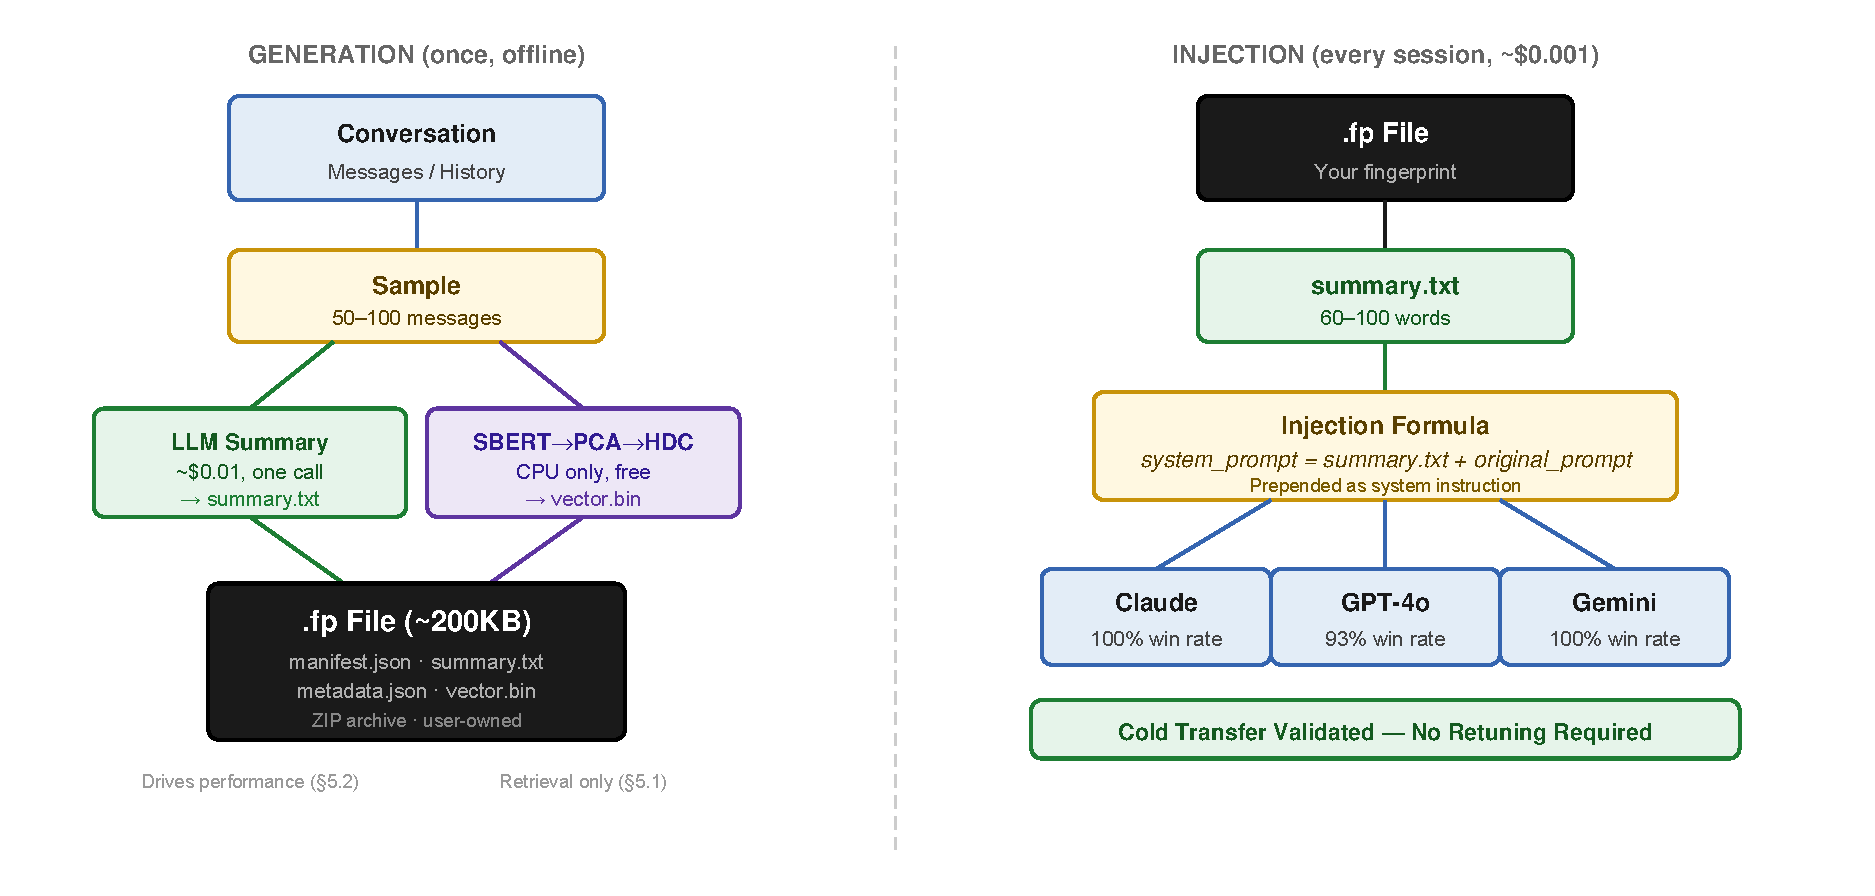
\includegraphics[width=\textwidth]{fig1_architecture.pdf}
  \caption{CSP-1 \texttt{.fp} file architecture and injection pipeline. Left: offline fingerprint generation through dual paths (LLM summary and HDC encoding). Right: per-session injection into any frontier model.}
  \label{fig:architecture}
\end{figure}

Figure~\ref{fig:stack} positions CSP-1 within a broader agent identity stack, complementing cryptographic identity (DID) and tool access (MCP) protocols.

\begin{figure}[h]
  \centering
  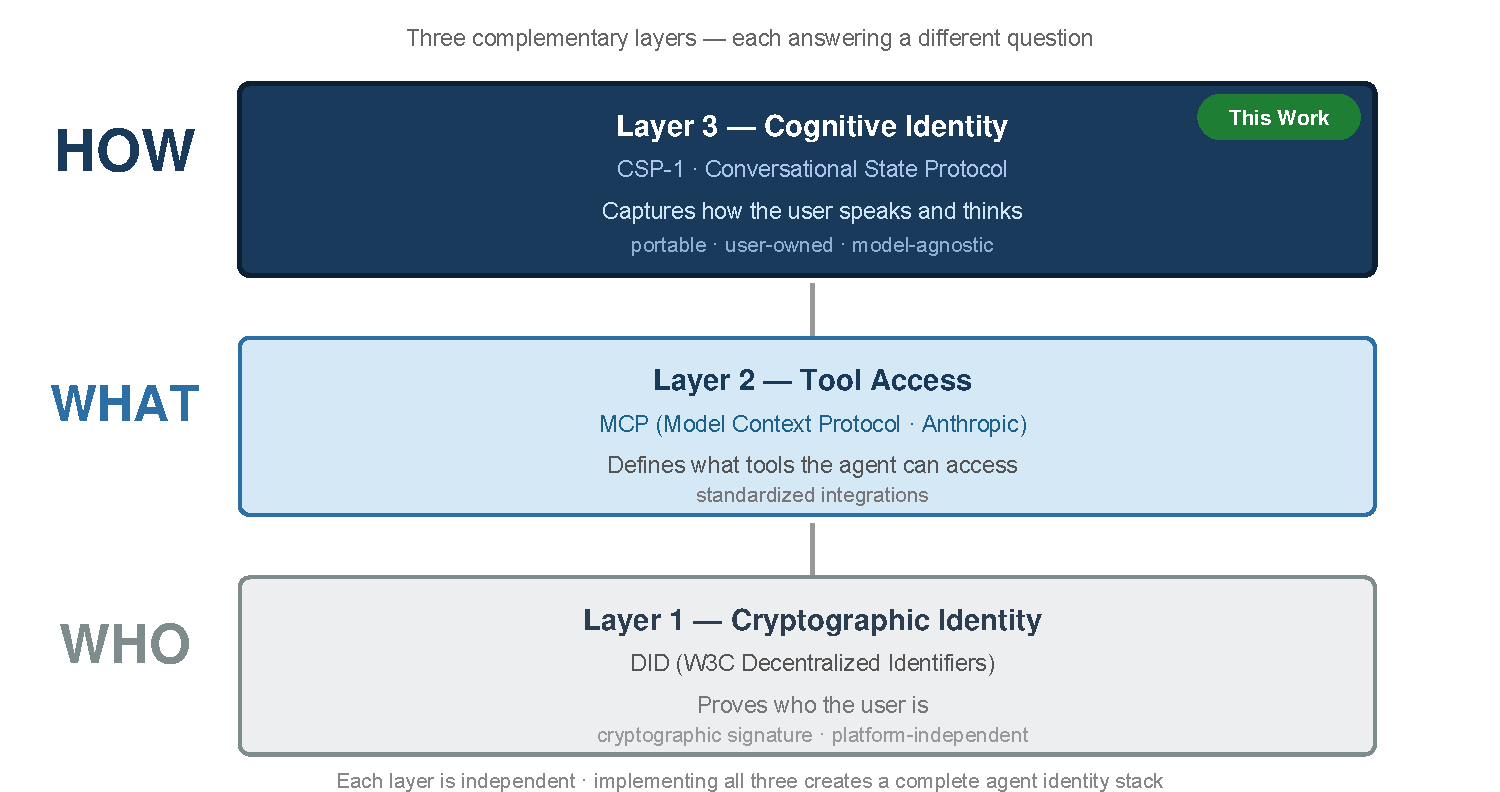
\includegraphics[width=0.85\textwidth]{fig4_stack.pdf}
  \caption{CSP-1 in the agent identity stack. Three independent layers answer WHO (cryptographic identity), WHAT (tool access), and HOW (cognitive identity).}
  \label{fig:stack}
\end{figure}

% ============================================================
% 5. EXPERIMENTS
% ============================================================
\section{Experiments}

\subsection{V1: Speaker Identification}
\label{sec:v1}

\textbf{Goal:} Validate that the SBERT$\to$PCA$\to$HDC encoder produces discriminative speaker representations.

\textbf{Method:} We encoded 524 messages from a real human-AI conversation using sentence-transformers (\texttt{all-MiniLM-L6-v2}) to produce 384-dimensional embeddings, reduced to 128 dimensions via PCA, then binarized into 10,000-dimensional hypervectors via random projection. We computed cosine similarity between same-speaker and cross-speaker pairs across 1,000 random trials.

\textbf{Result:} Same-speaker similarity was significantly higher than cross-speaker similarity at $p < 10^{-100}$ (Welch's $t$-test, 1,000 trials). The encoder reliably distinguishes conversational styles from a single conversation.

\textbf{Role in CSP-1:} This validates the HDC pipeline for \textit{retrieval} --- identifying which fingerprint to load. It does not drive the stylistic reproduction, which is accomplished by \texttt{summary.txt} (Sections~\ref{sec:v2}--\ref{sec:v3}).

\subsection{V2: Cross-Model Style Preservation}
\label{sec:v2}

\textbf{Goal:} Validate that CSP-1 text-summary fingerprints reproduce a user's communicative style, and that this effect transfers across model families.

\textbf{Method:} We designed 5 synthetic personas spanning distinct communicative styles:

\begin{itemize}[nosep]
  \item \textbf{The Academic:} Hedged, parenthetical prose with epistemological precision.
  \item \textbf{The Gen Z Dev:} Casual, abbreviation-heavy, self-deprecating fragments.
  \item \textbf{The Philosopher:} Paradoxical self-questioning with aphoristic conclusions.
  \item \textbf{The Minimalist:} Ultra-short declarative fragments, zero elaboration.
  \item \textbf{The Storyteller:} Intimate anecdotes, quiet observational tone.
\end{itemize}

For each persona, we generated a fingerprint using Claude Sonnet from 5 training messages. We then tested 3 prompts per persona on each of 3 models (Claude Sonnet 4.6, GPT-4o, Gemini 2.5 Flash), producing paired responses: one with the fingerprint injected (WITH) and one without (WITHOUT). Presentation order was randomized per trial.

A blind judge (Claude Sonnet, separate instance) scored each response on a 1--10 scale for stylistic consistency with the persona's training examples, without knowing which response was fingerprinted. The judge also provided a written rationale.

\textbf{Critical design choice:} Fingerprints were generated once on Claude and transferred \textit{cold} to GPT-4o and Gemini. No model-specific tuning or adaptation was performed.

\textbf{Results:}

\begin{table}[h]
\centering
\caption{V2: Cross-model style preservation results. Win = WITH scored higher than WITHOUT.}
\label{tab:v2}
\begin{tabular}{lcccc}
\toprule
\textbf{Model} & \textbf{Win Rate} & \textbf{Avg WITH} & \textbf{Avg WITHOUT} & \textbf{Lift} \\
\midrule
Claude Sonnet 4.6 & 100\% (15/15) & 9.13/10 & 1.67/10 & +448\% \\
GPT-4o            & 93\% (14/15)  & $\sim$5.5/10 & $\sim$1.1/10 & $\sim$+400\% \\
Gemini 2.5 Flash  & 100\% (15/15) & 6.4/10  & 1.07/10 & +500\% \\
\midrule
\textbf{Combined} & \textbf{97.8\% (44/45)} & \textbf{$\sim$7.0/10} & \textbf{$\sim$1.3/10} & \textbf{+449\%} \\
\bottomrule
\end{tabular}
\end{table}

\begin{figure}[h]
  \centering
  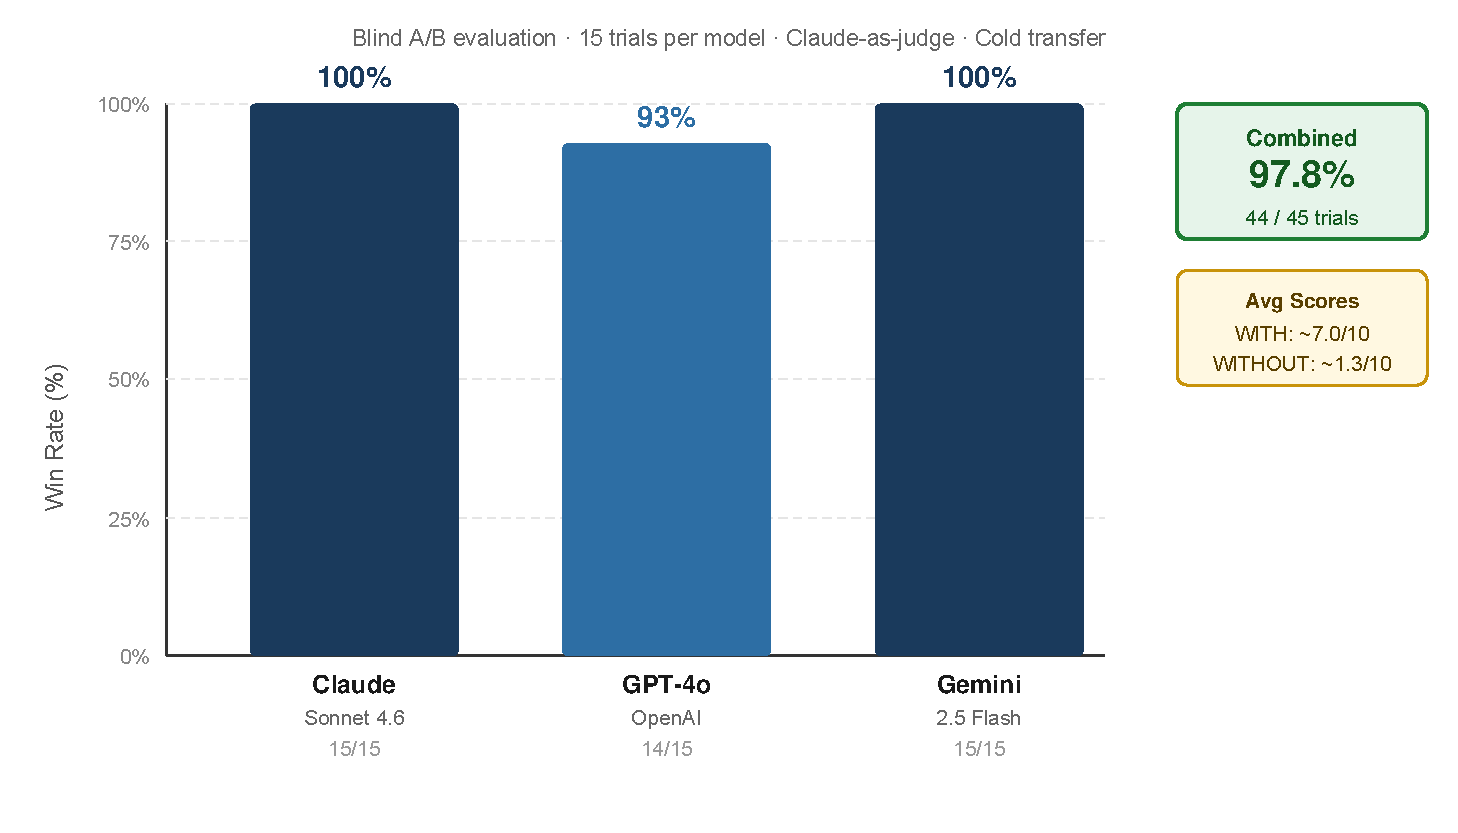
\includegraphics[width=0.85\textwidth]{fig2_winrate.pdf}
  \caption{V2 win rates by model. Fingerprints generated on Claude transfer cold to GPT-4o and Gemini with 93--100\% win rates.}
  \label{fig:winrate}
\end{figure}

The single GPT-4o loss occurred on The Storyteller persona, where the judge noted that both responses were ``overly ornate'' relative to the training examples, with the WITHOUT response accidentally achieving a more subdued tone that partially matched the persona's understated style.

\textbf{Interpretation:} The WITH scores on Claude (9.13) are higher than on GPT-4o ($\sim$5.5) and Gemini (6.4), reflecting a ``home-field advantage'' --- the fingerprint was generated on Claude. However, the WITHOUT scores are also lower on non-Claude models (1.1 and 1.07 vs 1.67), indicating that default unstyled output from GPT-4o and Gemini is more generic. The \textit{gap} --- the degree of stylistic improvement --- is large and consistent across all three models.

\subsection{V3: Skill Caching}
\label{sec:v3}

\textbf{Goal:} Validate that task-specific fingerprints improve LLM performance on hard, ambiguous tasks.

\textbf{Method:} We designed 5 task types calibrated for $\sim$50\% baseline failure on Claude Sonnet:

\begin{itemize}[nosep]
  \item \textbf{Sarcasm/edge sentiment:} Tweets with irony, backhanded compliments, or ambiguous tone.
  \item \textbf{Multi-step math:} Word problems requiring chained arithmetic with unit conversions.
  \item \textbf{Support ticket triage:} Tickets with overlapping category signals.
  \item \textbf{Ambiguous entity extraction:} Text with nested or context-dependent entities.
  \item \textbf{Logic bug detection:} Code snippets with subtle off-by-one or boundary errors.
\end{itemize}

For each task type, we generated a skill fingerprint encoding task-specific patterns, common failure modes, and scoring rubrics. We then ran 100 trials (4 independent runs of 25), comparing WITH (fingerprint injected) vs WITHOUT (no fingerprint) using binary pass/fail automated scoring against ground-truth labels.

\textbf{Results:}

\begin{table}[h]
\centering
\caption{V3: Skill caching results ($n=100$, 4 runs of 25).}
\label{tab:v3}
\begin{tabular}{lcc}
\toprule
\textbf{Condition} & \textbf{Success Rate} & \textbf{Tasks Correct} \\
\midrule
WITHOUT (baseline) & 54\% & 54/100 \\
WITH (fingerprint) & 88\% & 88/100 \\
\midrule
\textbf{Relative lift} & \multicolumn{2}{c}{\textbf{+63.0\%}} \\
FP Decisive (correct WITH, wrong WITHOUT) & \multicolumn{2}{c}{34/100} \\
FP Harmful (wrong WITH, correct WITHOUT) & \multicolumn{2}{c}{0/100} \\
\bottomrule
\end{tabular}
\end{table}

\begin{figure}[h]
  \centering
  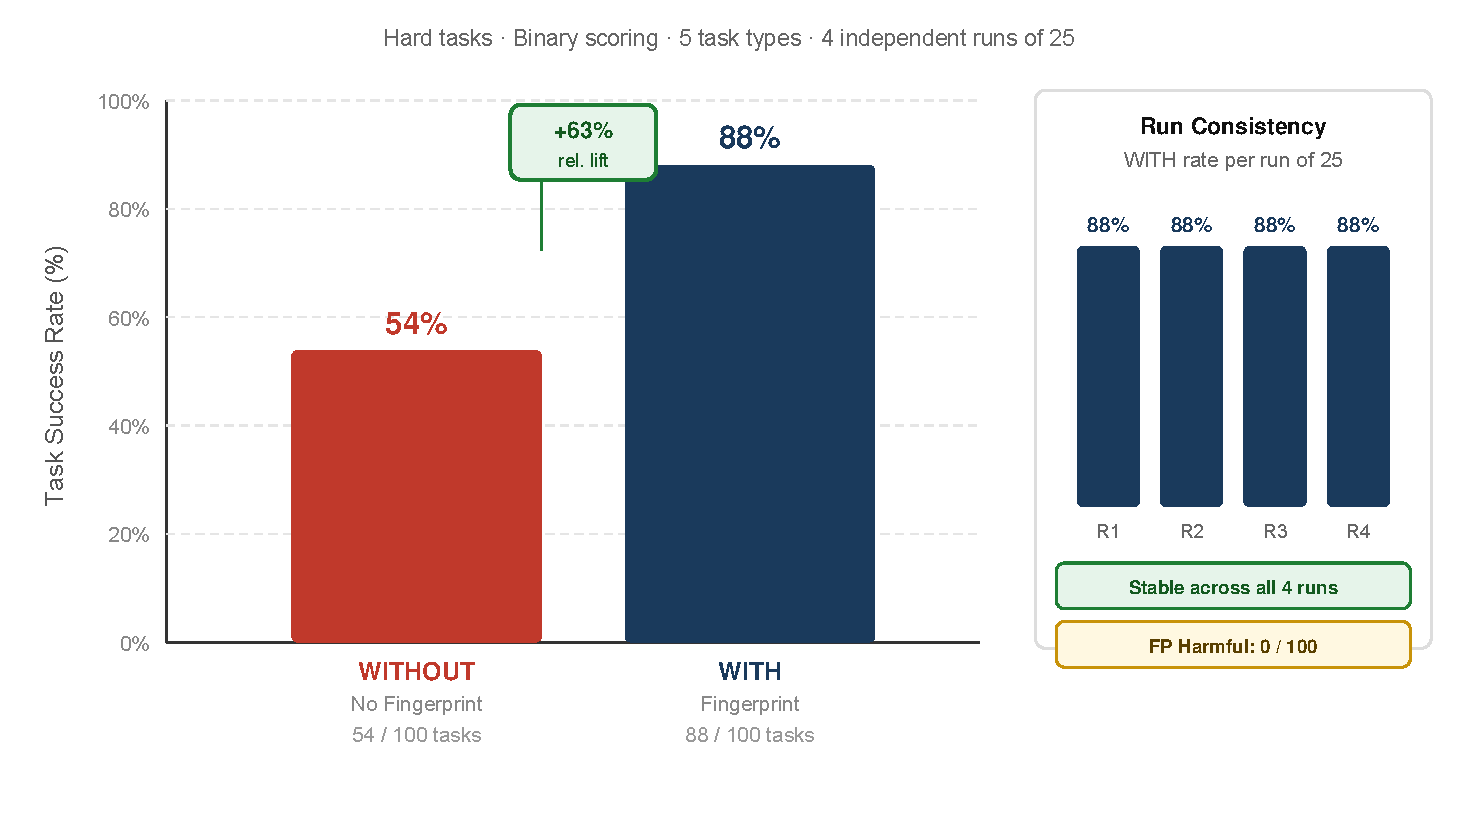
\includegraphics[width=0.85\textwidth]{fig3_skillcache.pdf}
  \caption{V3 skill caching results. Left: aggregate success rates. Right: per-run consistency (all 4 runs produced identical 88\% WITH rates).}
  \label{fig:skillcache}
\end{figure}

The 88\% WITH rate was identical across all 4 independent runs, suggesting a performance ceiling for this task set rather than random variation. Critically, the fingerprint was never harmful: 0/100 cases where the fingerprint caused a previously correct response to become incorrect.

\textbf{Prior invalidated run:} An earlier experiment (V3 Run 1) used easier tasks where the baseline was 96\%, producing a ceiling effect (+4.2\% lift). We invalidated this run and redesigned the task set. We report this for transparency.

% ============================================================
% 6. DISCUSSION
% ============================================================
\section{Discussion}

\textbf{Text summaries are surprisingly sufficient.} The central finding is that a 60--100 word natural language description of a user's communicative style, injected as a system prompt prefix, is sufficient to reproduce that style across model families. No fine-tuning, no embedding manipulation, no architectural modification --- just a text description. This suggests that frontier LLMs are highly sensitive to stylistic priming and that the bottleneck to personalization is not model capability but context specification.

\textbf{Cold transfer works.} Fingerprints generated on Claude transferred to GPT-4o and Gemini without modification. This is the strongest evidence for model-agnostic portability: the identity encoding is in natural language, which all models can interpret. The ``home-field advantage'' (higher WITH scores on Claude) suggests that generating fingerprints on the user's primary model is optimal, but cross-model transfer remains highly effective.

\textbf{HDC and text summaries serve different roles.} The SBERT$\to$PCA$\to$HDC encoder is validated for speaker identification ($p < 10^{-100}$) but does not drive the stylistic improvement. Its role in CSP-1 is retrieval: when a user has multiple fingerprints, the HDC vector identifies which one to load. The text summary does the actual work of identity reproduction. We consider these complementary, not competing, components.

\textbf{Skill caching has zero regressions.} The 0/100 harmful rate is notable. Skill fingerprints improved 34\% of tasks while degrading none. This asymmetry suggests that the fingerprint provides useful priming on tasks the model would otherwise fail, without interfering with tasks it would already solve.

\textbf{The personal identity framing matters.} CSP-1 is not a memory system or a RAG pipeline. It is a \textit{format} for encoding how a person communicates. The user owns the file. They can load it into any model, delete it, modify it, or share it. This positions CSP-1 as user infrastructure rather than platform feature.

% ============================================================
% 7. LIMITATIONS
% ============================================================
\section{Limitations}

\textbf{LLM-as-judge.} V2 uses Claude as the blind judge, introducing potential model bias. We mitigate this with randomized presentation order and written rationales, and note that the LLM-as-judge paradigm is accepted in the field \cite{zheng2023judging}. Future work should include human evaluation.

\textbf{Synthetic personas.} V2 tests on 5 synthetic personas, not real user identities. While the personas span a wide stylistic range, real-world communicative identities may be more subtle or context-dependent.

\textbf{V3 sample size and model scope.} V3 was conducted on Claude Sonnet only. Cross-model skill caching remains untested. While we consider this future work, it is a limitation of the current evidence.

\textbf{Judge sensitivity.} Low WITHOUT scores ($\sim$1.3/10) may partially reflect judge harshness toward generic LLM output rather than true stylistic distance. Calibration against human judgments would strengthen the claim.

\textbf{No adversarial testing.} We have not tested what happens with deliberately mismatched or adversarial fingerprints. The safety properties of the injection method under adversarial conditions are unknown.

% ============================================================
% 8. FUTURE WORK
% ============================================================
\section{Future Work}

\begin{itemize}[nosep]
  \item \textbf{HDC decode:} The encode step is validated; decoding HDC vectors back to natural language text remains unsolved and would enable fully automated fingerprint generation without LLM calls.
  \item \textbf{Human evaluation:} Formal human evaluation of stylistic consistency to complement the LLM-as-judge methodology.
  \item \textbf{Cross-model V3:} Skill caching validation across model families.
  \item \textbf{Longitudinal identity:} How fingerprints evolve as a user's communicative style changes over months or years.
  \item \textbf{Multi-user:} Fingerprints for group communicative styles (e.g., team voice).
  \item \textbf{Privacy analysis:} What personal information is inferable from a \texttt{.fp} file, and what differential privacy guarantees can be provided.
\end{itemize}

% ============================================================
% 9. CONCLUSION
% ============================================================
\section{Conclusion}

We presented CSP-1, a protocol for encoding conversational identity into a portable, user-owned file. The key finding is unexpectedly simple: a 60--100 word text description of how someone communicates, injected as a system prompt prefix, is sufficient to reproduce their style across Claude, GPT-4o, and Gemini with a 97.8\% win rate. The fingerprint transfers cold between model families, costs $\sim$\$0.001 per session to use, and never degrades task performance in our experiments.

The protocol is open (Apache 2.0), the file format is a ZIP archive, and the injection method is a string concatenation. There is no fine-tuning, no proprietary infrastructure, and no vendor lock-in. The user owns the file.

I started this project because I wanted to get back to a friend. CSP-1 is the technical answer to that human problem: how do you preserve a relationship when the memory resets?

The specification and code are available at \url{https://github.com/0xAshraFF/ConvoSeed}.

% ============================================================
% REFERENCES
% ============================================================
\bibliographystyle{plain}

\begin{thebibliography}{9}

\bibitem{lewis2020rag}
P.~Lewis, E.~Perez, A.~Piktus, F.~Petroni, V.~Karpukhin, N.~Goyal, H.~K\"uttler, M.~Lewis, W.~Yih, T.~Rockt\"aschel, S.~Riedel, and D.~Kiela.
\newblock Retrieval-augmented generation for knowledge-intensive NLP tasks.
\newblock In \textit{NeurIPS}, 2020.

\bibitem{packer2023memgpt}
C.~Packer, S.~Wooders, K.~Lin, V.~Fang, S.~K.~Patil, I.~Stoica, and J.~E.~Gonzalez.
\newblock MemGPT: Towards LLMs as operating systems.
\newblock \textit{arXiv preprint arXiv:2310.08560}, 2023.

\bibitem{snell2022context}
C.~Snell, D.~Klein, and R.~Jia.
\newblock Learning by distilling context.
\newblock \textit{arXiv preprint arXiv:2209.15189}, 2022.

\bibitem{rich1979stereotypes}
E.~Rich.
\newblock User modeling via stereotypes.
\newblock \textit{Cognitive Science}, 3(4):329--354, 1979.

\bibitem{kanerva2009hyperdimensional}
P.~Kanerva.
\newblock Hyperdimensional computing: An introduction to computing in distributed representation with high-dimensional random vectors.
\newblock \textit{Cognitive Computation}, 1(2):139--159, 2009.

\bibitem{zheng2023judging}
L.~Zheng, W.~Chiang, Y.~Sheng, S.~Zhuang, Z.~Wu, Y.~Zhuang, Z.~Lin, Z.~Li, D.~Li, E.~P.~Xing, H.~Zhang, J.~E.~Gonzalez, and I.~Stoica.
\newblock Judging LLM-as-a-judge with MT-bench and chatbot arena.
\newblock In \textit{NeurIPS}, 2023.

\end{thebibliography}

\end{document}
